\documentclass[11pt,a4paper]{article}
\usepackage{times}
\usepackage{natbib}
\setcitestyle{round, authoryear}
\usepackage{amssymb}
\usepackage{amsmath}
\newcommand*\diff{\mathop{}\!\mathrm{d}}
\DeclareMathOperator*{\argmax}{arg\,max}
\usepackage{subfig}

\title{Optimizing Discrete Units in Stochastic Computation Graphs}

\usepackage{natbib}
\usepackage{graphicx}

\begin{document}

\maketitle


Consider a stochastic computation graph (SCG), where $X$ is a hidden stochastic layer (backpropagation covers the rest). We can interpret the forward pass in the graph as first sampling $x$ from the conditional distribution $p_\phi(x)$ of $X$ given its parent layers, then evaluate a deterministic function $f_\theta(x)$ at $X$. We can think of $f_\theta(x)$ as a noisy objective, so we are interested in optimizing its expected value $L(\theta, \phi) = \mathbb{E}_{x\sim p_\phi(x)}[f_\theta(x)]$ w.r.t. parameters $\theta, \phi$.

In general, the gradient w.r.t. the parameters $\theta$ is given as:
\begin{equation}
    \nabla_\theta L(\theta, \phi) = \nabla_\theta \mathbb{E}_{x\sim p_\phi(x)}[f_\theta(x)] = \mathbb{E}_{x\sim p_\phi(x)}[\nabla_\theta f_\theta(x)]
\end{equation}
and can be estimated by Monte Carlo sampling:
\begin{equation}
    \nabla_\theta L(\theta, \phi) \simeq \frac{1}{S} \sum_{s=1}^{S} \nabla_\theta f_\theta(x^{s})
\end{equation}
where $x^{s} \sim p_\phi(x)$ i.i.d. 

The challenging task is to compute the gradient w.r.t. the parameters $\phi$ of $p_\phi(x)$.
The expression
\begin{equation}
\label{grad}
    \nabla_\phi L(\theta, \phi) = \nabla_\phi \int p_\phi(x) f_\theta(x) \diff x = \int f_\theta(x) \nabla_\phi p_\phi(x) \diff x 
\end{equation}
does not have the form of an expectation w.r.t. $x$ and consequently does not lead to a Monte Carlo gradient estimator. However, there are two ways of tackling this problem.


\section{Score Function Estimators}


The score function estimator (SFE, \cite{fu2006gradient}), also known as the REINFORCE \citep{williams1992simple} or likelihood-ratio estimator \citep{glynn1990likelihood}, is based on the identity 
\begin{equation}
    \nabla_\phi p_\phi(x) = p_\phi(x) \nabla_\phi \log p_\phi(x) ,
\end{equation}
which allows the gradient in Equation (\ref{grad}) to be written as 
\begin{align}
\begin{split}
    \nabla_\phi L(\theta, \phi) & = \nabla_\phi \int f_\theta(x) p_\phi(x) \diff x \\
    & = \int f_\theta(x) \nabla_\phi p_\phi(x) \diff x \\
    & = \int f_\theta(x) p_\phi(x) \nabla_\phi \log p_\phi(x) \diff x \\
    & = \mathbb{E}_{x\sim p_\phi(x)}[f_\theta(x) \nabla_\phi \log p_\phi(x)]
\end{split}
\end{align}
We can then estimate this gradient via Monte Carlo sampling
\begin{equation}
    \nabla_\phi L(\theta, \phi) \simeq \frac{1}{S} \sum_{s=1}^{S} f_\theta(x^{s}) \nabla_\phi \log p_\phi(x^{s})
\end{equation}
where $x^{s} \sim p_\phi(x)$ i.i.d. As it does not require $f_\theta(x)$ to be differentiable or even continuous as a function of $x$, the SFE can be used for both continuous and discrete random variables.

Though the basic version of the estimator suffers from high variance, various variance reduction techniques are used to make the estimator much more effective. Baselines are the most important and widely used of these techniques \citep{williams1992simple}. Specifically, a control variate $b(x)$ can be subtracted from the learning signal $f_\theta(x)$ and its analytical expectation $\mu_b = \mathbb{E}_{x\sim p_\phi(x)}[b(x)\nabla_\phi \log p_\phi(x)] $ should also be added back to keep the estimator unbiased:
\begin{equation}
    \nabla_\phi L(\theta, \phi) = \mathbb{E}_{x\sim p_\phi(x)}[(f_\theta(x) - b(x))\nabla_\phi \log p_\phi(x)] + \mu_b 
\end{equation}

Here we briefly summarize recent stochastic gradient estimators that utilize control variates.

\paragraph{NVIL \citep{mnih2014neural}} uses two baselines: (1) a moving average $\bar{f}$ of $f$ to center the learning signal, and (2) an input-dependent baseline computed by a neural network (a control variate for the centered learning signal itself). Finally, variance normalization divides the learning signal by $\max(1,\sigma_f)$, where $\sigma_f^2$ is a moving average of $\text{Var}[f]$. We will discuss more about NVIL in the context of variational inference.

\paragraph{DARN \citep{gregor2013deep}} uses $b = f(\bar{x}) + f'(\bar{x})(x - \bar{x})$, where the baseline corresponds to the first-order Taylor approximation of $f(x)$ from $f(\bar{x})$. $x$ is chosen to be 1/2 for Bernoulli variables, which makes the estimator biased for non-quadratic $f$, since it ignores the correction term $\mu_b$ in the estimator expression.

\paragraph{MuProp \citep{gu2015muprop}} also models the baseline as a first-order Taylor expansion: $b = f(\bar{x}) + f'(\bar{x})(x - \bar{x})$ and $\mu_b = f'(\bar{x})\nabla\phi \mathbb{E}_{x\sim p_\phi(x)} [x]$. To overcome backpropagation through discrete sampling, a mean-field approximation $f_{MF} (\mu_\phi(x))$ is used in place of $f(x)$ to compute the baseline and derive the relevant gradients.

\paragraph{VIMCO \citep{mnih2016variational}} is a gradient estimator for multi-sample objectives that uses the mean of other samples $b = \frac{1}{m}\sum_{j\neq i} f(x_j)$ to construct a baseline for each sample $x_i \in x_{1:m}$.

\section{Reparameterization Trick}

In many cases we can sample from $p_\phi(x)$ by first sampling $z$ from some fixed distribution $q(z)$ and then transforming the sample using some function $g_\phi(z)$. For example, a sample from $\text{Normal}(\mu,\sigma^2)$ can be obtained by sampling $z$ from the standard form of the distribution $\text{Normal}(0, 1)$ and then transforming it using $g_{\mu,\sigma}(z) = \mu + \sigma z$. This two-stage reformulation of the sampling process, called the reparameterization trick, allows us to transfer the dependence on $\phi$ from $p$ into $f$ by writing $f_\theta(x) = f_\theta(g_\phi(z))$ for $x = g_\phi(z)$, making it possible to reduce the problem of estimating the gradient w.r.t. parameters of a distribution to the simpler problem of estimating the gradient w.r.t. parameters of a deterministic function.

Having reparameterized $p_\theta(x)$, we can now express the objective as an expectation w.r.t. $q(z)$
\begin{equation}
   L(\theta, \phi) = \mathbb{E}_{x \sim p_\phi(x)}[f_\theta(x)] = \mathbb{E}_{z \sim q_\phi(z)}[f_\theta(g(z))]
\end{equation}
As $q(z)$ does not depend on $\phi$, we can estimate the gradient w.r.t. $\phi$ in exactly the same way we estimated the gradient w.r.t. $\theta$.


\subsection{Gumbel-Softmax}
In the case of categorical variables, reparameterization trick cannot be applied directly. \citet{maddison2016concrete, jang2016categorical} proposed Gumbel-Softmax (also known as Concrete distribution) to replace the non-differentiable samples from a categorical distribution with differentiable samples from a Gumbel-Softmax distribution.

The Gumbel-Softmax distribution is motivated from the Gumbel-Max trick. Consider an unnormalized parameterization $(\alpha_1,...,\alpha_n)$ where $\alpha_k \in (0,\infty)$ of a discrete distribution $D \sim \text{Discrete}(\alpha)$. We assume that states with 0 probability are excluded. The Gumbel-Max trick proceeds as follows: sample $u_k \sim \text{Uniform}(0, 1)$ i.i.d. for each $k$, find $k$ that maximizes ${\log\alpha_k -\log(-\log u_k)}$, set $D_k = 1$ and the remaining $D_i = 0$ for $i \neq k$. Then
\begin{equation}
    \mathbb{P}(D_k = 1) = \frac{\alpha_k}{\sum_{i=1}^{n}\alpha_i}
\end{equation}

In other words, the sampling of a discrete random variable can be refactored into a deterministic  function---componentwise addition followed by $\argmax$ of the parameters $\log \alpha_k$ and fixed distribution $-\log(-\log U_k)$. See Figure \ref{fig:gm} for a visualization.

\begin{figure}[htbp]
\centering
\subfloat[Gumbel-Max.\label{fig:gm}]
    {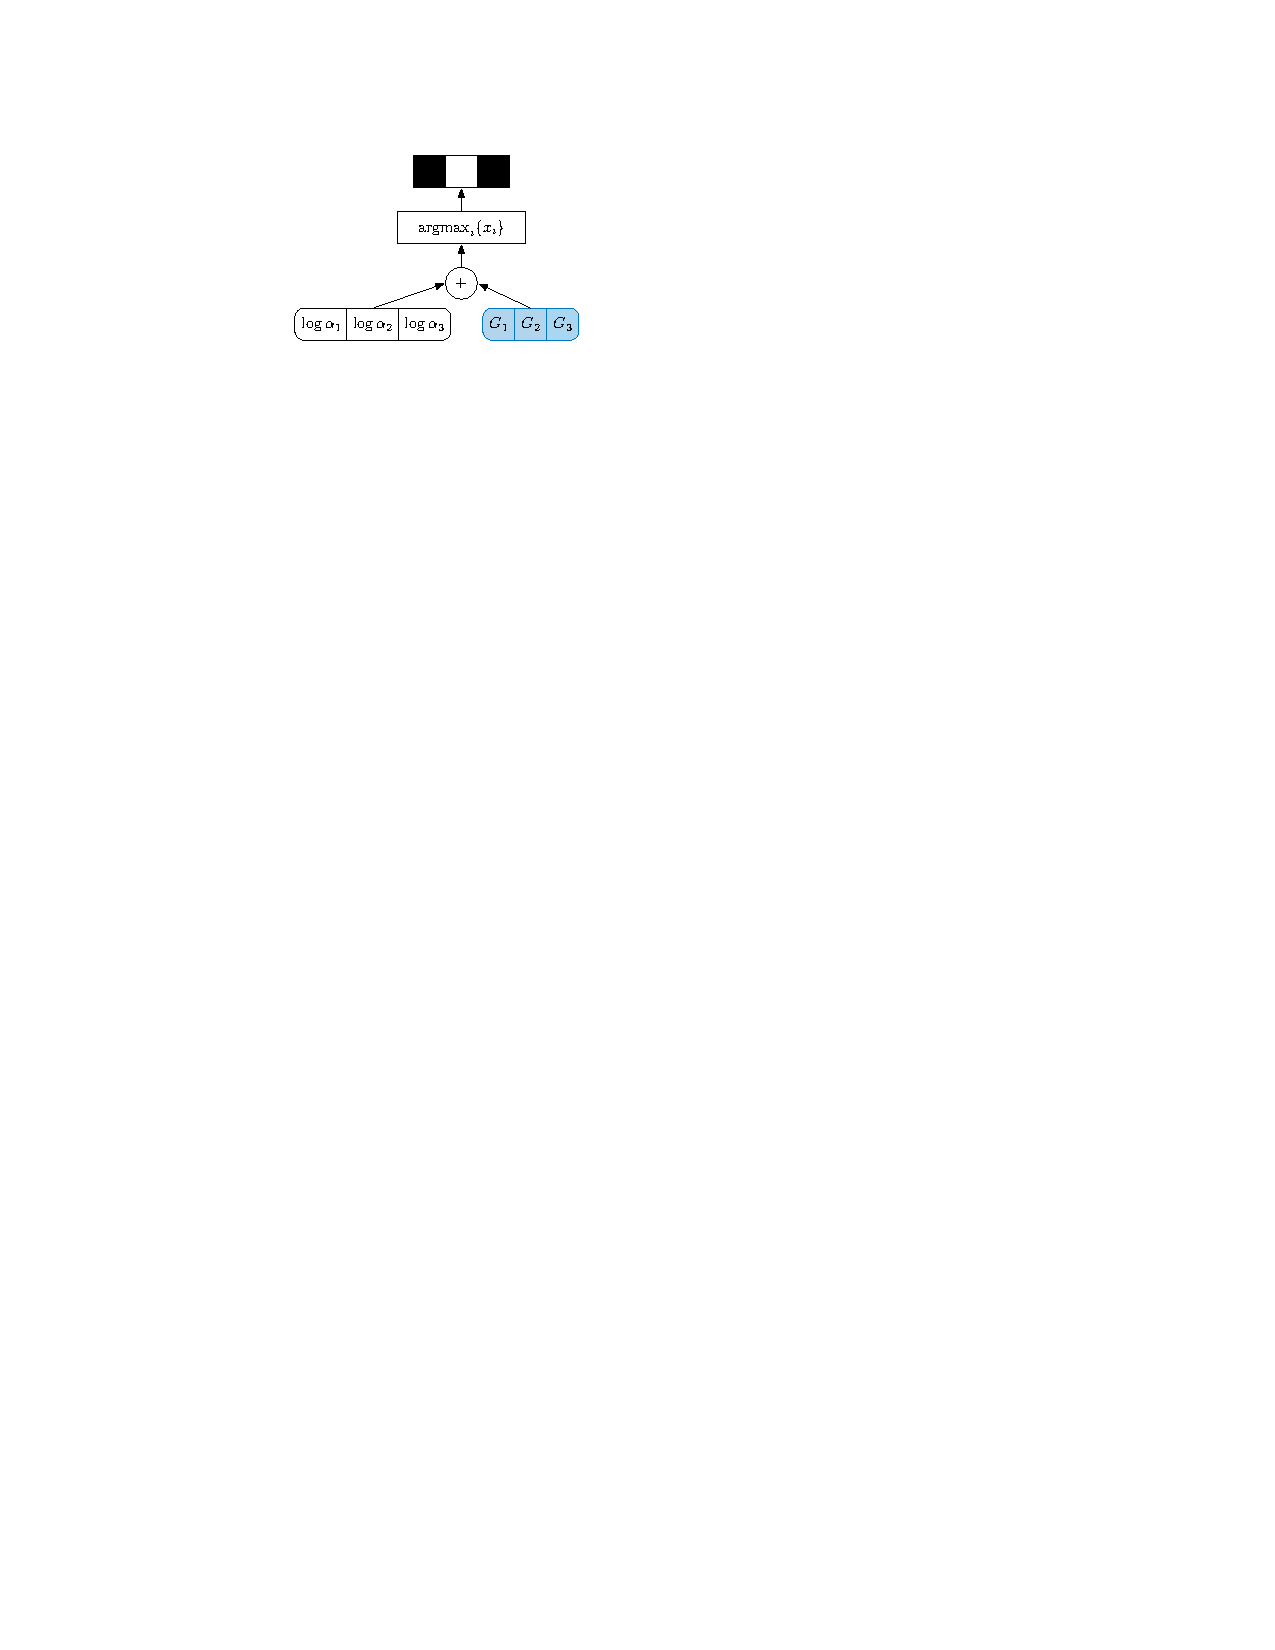
\includegraphics[width=0.46\textwidth]{Gumbel_max.pdf}}\hfill
\subfloat[Gumbel-Softmax.\label{fig:gs}]
    {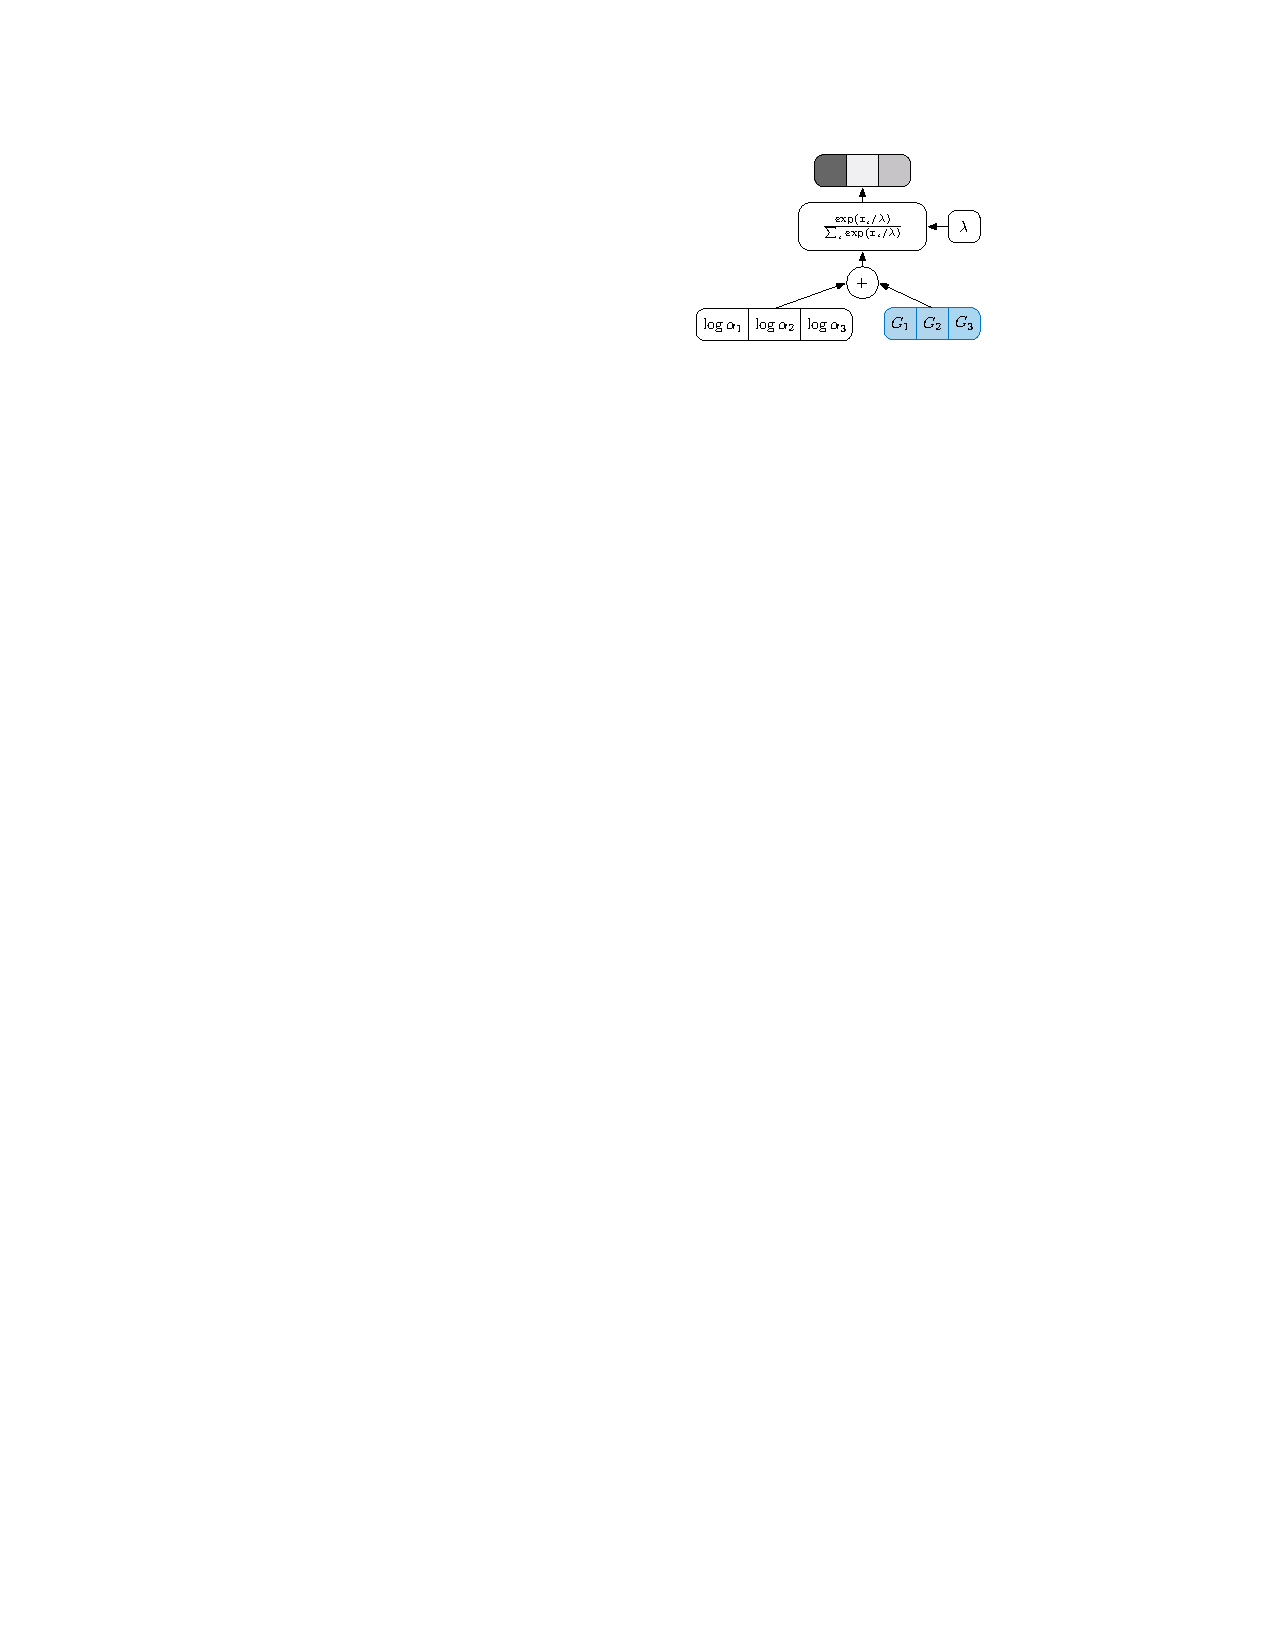
\includegraphics[width=0.46\textwidth]{Gumbel_softmax.pdf}}
    \caption{From \citet{maddison2016concrete}.}
\end{figure}

The $\argmax$ computation returns states on the vertices of the simplex $\Delta^{n-1} = \{ x \in \mathbb{R}^n | x_k \in [0, 1],\sum_{k=1}^{n} x_k = 1 \} $. Then the state of a discrete variable can be relaxed from the vertices into the interior where it is a random probability vector using Softmax. To sample a Gumbel-Softmax random variable $x \in \Delta^{n-1}$ at temperature $\lambda \in (0,\infty)$ with parameters $\alpha_k \in (0,\infty)$, sample $G_k \sim \text{Gumbel}$ i.i.d. and set
\begin{equation}
\label{Gumbel-Softmax}
    x_k = \frac{\exp{((\log \alpha_k + G_k) / \lambda})}{\sum_{i=1}^{n} \exp{((\log \alpha_k + G_k) / \lambda})}
\end{equation}

The Gumbel-Softmax computation of Equation (\ref{Gumbel-Softmax}) smoothly approaches the discrete $\argmax$ computation as $\lambda \to 0$ while preserving the relative order of the Gumbels $\log \alpha_k + G_k$.

While Gumbel-Softmax samples are differentiable, they are not identical to samples from the corresponding categorical distribution for non-zero temperature. For learning, there is a tradeoff between small temperatures, where samples are close to one-hot but the variance of the gradients is large, and large temperatures, where samples are smooth but the variance of the gradients is small. In practice, the temperature can be set high initially and is annealed to small but non-zero as the training proceeds. If $\lambda$ is a learned parameter (rather than annealed via a fixed schedule), this scheme can be interpreted as entropy regularization , where the Gumbel-Softmax distribution can adaptively adjust the ``confidence'' of proposed samples during the training process.

For scenarios in which we are constrained to sampling discrete values, we discretize $x$ using $\argmax$ in the forward pass but use the continuous approximation in the backward pass. It is called the Straight-Through (ST) Gumbel Estimator.


\section{Application on Variational Training of Categorical Latent Variable Models}


Hidden variable models assume that each observation $x$ is obtained by first sampling a vector of categorical latent variables $z$ and then generating the observation itself by sampling from $p_\theta(x|z)$ or a deterministic decoder $f_\theta(z)$. \footnote{One can also model the joint distribution $p(x,z)$ directly if the factorization into $p(z)$ and $p(x|z)$ is infeasible, although this model  } 

The data log likelihood can be written as 
\begin{align}
    \begin{split}
        L(\theta) & = \log \mathbb{E}_{z \sim p_\theta(z)} [p_\theta(x|z)] \\
        & = \log \sum_z p_\theta(x,z).
    \end{split}
\end{align}
This is typically intractable and does not fit into the previous SCG framework due to the expectation being inside the $\log$. Alternatively, it is widely used to optimize evidence lower bound (ELBO) on data log likelihood
\begin{equation}
    \begin{split}
        L(\theta) & = \log \sum_z p_\theta(x,z) \\
        & = \sum_z Q_\phi(z|x) \log \frac{p_\theta(x,z)}{Q_\phi(z|x)} + KL[Q_\phi(z|x), p(z|x)].
    \end{split}
\end{equation}
The ELBO can be written as 
\begin{align}
\label{ELBO}
    \begin{split}
        \mathcal{L}(x, \theta, \phi) = & \sum_z Q_\phi(z|x) \log \frac{p_\theta(x,z)}{Q_\phi(z|x)} \\
            & = \mathbb{E}_{z \sim Q_\phi(z|x)} [\log p_\theta(x,z) - \log Q_\phi(z|x)].
    \end{split}
\end{align}


\subsection{Revisiting NVIL}


NVIL proposed a baseline based variance reduction technique for neural variational inference on categorical variables. 
$\log p_\theta(x,z) - \log Q_\phi(z|x)$ in Equation (\ref{ELBO}) can viewed as the learning signal from the perspective of reinforcement learning, especially policy gradient. 

In SFE, the gradient of the parameters $\phi$ can be estimated as

\begin{align}
\label{signal}
    \begin{split}
        \nabla_\phi \mathcal{L} & = \nabla_\phi \sum_z  Q_\phi(z|x) ( \log p_\theta(x,z) - \log Q_\phi(z|x) ) \\
        & = \sum_z \log p_\theta(x,z) \nabla_\phi Q_\phi(z|x) - \nabla_\phi \sum_z Q_\phi(z|x) \log Q_\phi(z|x) \\
        & = \sum_z \log p_\theta(x,z) \nabla_\phi Q_\phi(z|x) - \sum_z ( \log Q_\phi(z|x) \nabla_\phi Q_\phi(z|x) + \nabla_\phi Q_\phi(z|x) ) \\
        & = \sum_z ( \log p_\theta(x,z) - \log Q_\phi(z|x) ) \nabla_\phi Q_\phi(z|x) \\
        & = \sum_z ( \log p_\theta(x,z) - \log Q_\phi(z|x) ) Q_\phi(z|x) \nabla_\phi \log Q_\phi(z|x)\\
        & = \mathbb{E}_{z \sim Q_\phi(z|x)} [(\log p_\theta(x,z) - \log Q_\phi(z|x))  \nabla_\phi \log Q_\phi(z|x)]
    \end{split}
\end{align}

It might be surprising that this learning signal will fit $Q_\phi(z|x)$ to $p_\theta(x,z)$ other than the true posterior $p(z|x)$.

And since
\begin{align}
    \begin{split}
        \mathbb{E}_{z \sim Q_\phi(z|x)} \nabla_\phi \log Q_\phi(z|x) & = \mathbb{E}_{z \sim Q_\phi(z|x)} \frac{\nabla_\phi Q_\phi(z|x)}{Q_\phi(z|x)}\\
        & = \sum_z \nabla_\phi Q_\phi(z|x) \\
        & = \nabla_\phi \sum_z  Q_\phi(z|x) \\
        & = 0 
    \end{split}
\end{align}
we can subtract any $c$ that does not depend on $z$ from the learning signal in Equation (\ref{signal}).  However, $c$ will not be able capture the systematic differences in the learning signal for different observation $x$. Thus we can reduce the gradient variance further by subtracting an observation-dependent term $c_\psi(x)$ to minimize those differences. Note that, doing this will not affect the expectation in Equation (\ref{signal}), because $c_\psi(x)$ is independent on $z$. $c_\psi(x)$ can be implemented using a neural network and train it to minimize the expected square of the centered learning signal $\mathbb{E}_{z \sim Q_\phi(z|x)} [(\log p_\theta(x,z) - \log Q_\phi(z|x) - c_\psi(x) - c)^2]$.

In practice, using $\log p_\theta(x,z) - \log Q_\phi(z|x)$ as the learning signal is non-trivial as its average magnitude can change dramatically. NVIL addresses this issue by dividing the centered learning signal by a running estimate of its standard deviation in a mini-batch. This normalization ensures that the signal is approximately unit variance, and can be seen as a simple and efficient way of adapting the learning rate. To ensure that training will be stopped when the magnitude of the signal approaches zero, variance normalization will only be applied when the estimate of the standard deviation is greater than 1.

\bibliographystyle{abbrvnat}
\bibliography{references}
\end{document}
